%%%%%%%%%%%%%%%%%%%%%%%%%%%%%%%%%%%%%%%%%%%%%%%%%%%%%%%%%%%%%%%%%%%%%%%%%%%%%%%%
% oscillation_analysis.tex: Analysis of Neutrino Oscillations:
%%%%%%%%%%%%%%%%%%%%%%%%%%%%%%%%%%%%%%%%%%%%%%%%%%%%%%%%%%%%%%%%%%%%%%%%%%%%%%%%
\chapter{Group Problem}
\label{Group Problem}
%%%%%%%%%%%%%%%%%%%%%%%%%%%%%%%%%%%%%%%%%%%%%%%%%%%%%%%%%%%%%%%%%%%%%%%%%%%%%%%%
initial height h = 1.20 m\newline
ramp angle $\theta$ = 10 degrees\newline
empty barrel mass $M_{bar}$ = 13.5 kg, beer mass $M_{beer}$ = 59.3 kg\newline
force of friction $F_{f} = \mu N_{y}$\newline
gravity g = $9.81 \frac{m}{s^{2}}$\newline
barrel radius $r_{bar}$ = 0.215 m\newline
translational acceleration of barrel CM $a_{lin}$\newline
barrel angular acceleration $\alpha$\newline

a. force diagram shown in Figure \ref{fig:barrelOnRamp}\newline

\begin{figure}[h]
	\centering
	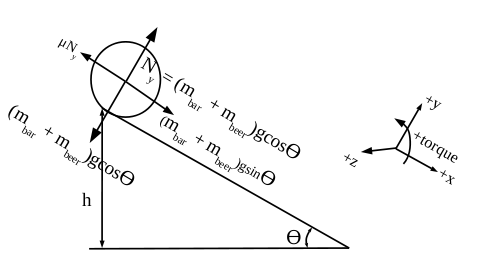
\includegraphics[width=0.7\textwidth]{figures/exam4groupProblemPartA.png}
	\caption{barrel rolling down ramp}
	\label{fig:barrelOnRamp}
\end{figure}

b. the torque on the barrel is -4.2 Nm (clockwise rotation)\newline
The only torque about the axis of rotation is created by friction $F_{f}$.  If the barrel rolls\newline
without slipping, then the linear acceleration $a_{lin}$ of the system center of mass\newline
in the x direction must be equal to $r_{bar} |\alpha|$.\newline
first solve for $a_{lin}$ in terms of $F_{f}$:\newline
$(M_{bar} + M_{beer})a_{lin} = (M_{bar} + M_{beer})g\sin(\theta) - F_{f}$\newline
$a_{lin} = g\sin(\theta) - \frac{F_{f}}{M_{bar} + M_{beer}} = r_{bar} |\alpha|$\newline

now solve for $\alpha$ in terms of $F_{f}$:\newline
torque about axis of rotation = -$F_{f}r_{bar}$ = $M_{bar}r_{bar}^{2} \alpha$\newline
note that only the mass of the barrel contributes to the moment of inertia of the\newline
keg; the beer in the keg does not rotate.\newline
$\alpha$ = -$\frac{r_{bar}}{M_{bar}r_{bar}^{2}} F_{f}$\newline

so equating $r_{bar} |\alpha|$ to $a_{lin}$ yields an expression for $F_{f}$\newline
$\frac{r_{bar}^{2}}{M_{bar}r_{bar}^{2}} F_{f} = g\sin(\theta) - \frac{F_{f}}{M_{bar} + M_{beer}}$\newline
or $F_{f}(\frac{1}{M_{bar} + M_{beer}} + \frac{1}{M_{bar}}) = g\sin(\theta)$\newline
thus $F_{f}$ = 19.40 N, and the torque on the barrel is -$F_{f}r_{bar}$ = -4.17 Nm\newline

c. \newline
linear accel $a_{lin} = g\sin(\theta) - \frac{1}{M_{bar} + M_{beer}}F_{f} = 1.44 \frac{m}{s^{2}}$\newline
ang accel $\alpha = -\frac{|a_{lin}|}{r_{bar}} = -6.68 \frac{rad}{s^{2}}$\newline

d. \newline
final linear velocity $v_{f} = \sqrt{2a_{lin}(1.20 / \sin(\theta) )} = 4.5 \frac{m}{s}$\newline
final angular velocity $\omega_{f} = -\frac{v_{f}}{r_{bar}} = -21 \frac{rad}{s}$\newline
final angular KE of barrel = $\frac{1}{2}M_{bar}r_{bar}^{2} \omega_{f}^{2}$ = 134 Joules\newline
final linear KE of barrel and beer = $\frac{1}{2}(M_{bar} + M_{beer}) v_{f}^{2}$ = 723 Joules\newline
another acceptable answer for the final linear KE is that of just the barrel, ignoring\newline
the mass of the beer.\newline
final linear KE of barrel only = $\frac{1}{2}M_{bar} v_{f}^{2}$ = 134 Joules\newline

e. the barrel rolls down the ramp in 3.0 seconds\newline
there are several ways to calculate the time required for the keg to roll down\newline
the ramp; two methods are shown here.\newline
after a time T the linear velocity is equal to the final linear velocity\newline
$v_{f} = 0 + a_{lin}T \rightarrow T = \frac{v_{f}}{a_{lin}}$ = 3.10 s\newline

the total angular distance travelled $\theta_{tot}$ is equal to half of\newline
the angular acceleration multiplied by $T^{2}$\newline
$\theta_{tot} = -\frac{6.28 rads}{revolution} \frac{1 revolution}{6.28r_{bar}} \frac{1.20 m}{\sin(\theta)}$\newline
$\theta_{tot}$ = -32.142 radians\newline
$\theta_{tot} = \frac{1}{2} \alpha T^{2}$\newline
so T = $\sqrt{\frac{2 \theta_{tot}}{\alpha}}$ = 3.10 s


%%%%%%%%%%%%%%%%%%%%%%%%%%%%%%%%%%%%%%%%%%%%%%%%%%%%%%%%%%%%%%%%%%%%%%%%%%%%%}}}
